\documentclass[conference]{IEEEtran}
\IEEEoverridecommandlockouts
% The preceding line is only needed to identify funding in the first footnote. If that is unneeded, please comment it out.
\usepackage{cite}
\usepackage{amsmath,amssymb,amsfonts}
\usepackage{algorithmic}
\usepackage{graphicx}
\usepackage{textcomp}
\usepackage{xcolor}
\usepackage{listings}
\def\BibTeX{{\rm B\kern-.05em{\sc i\kern-.025em b}\kern-.08em
    T\kern-.1667em\lower.7ex\hbox{E}\kern-.125emX}}

\definecolor{keywords}{RGB}{255,0,90}
\definecolor{comments}{RGB}{0,0,113}
\definecolor{red}{RGB}{160,0,0}
\definecolor{green}{RGB}{0,150,0}
\begin{document}

\lstset{language=Python, 
        basicstyle=\ttfamily\small, 
        keywordstyle=\color{keywords},
        commentstyle=\color{comments},
                stringstyle=\color{red},
        showstringspaces=false,
        identifierstyle=\color{green},
        keywords=[2]{pow},
        keywordstyle=[2]{\color{orange}},
}
\lstset{frame=lines}
%\lstset{caption={Insert code directly in your document}}
\lstset{label={lst:code_direct}}
\lstset{basicstyle=\footnotesize}


\title{MQTT\_Exercise\\
}

\author{\IEEEauthorblockN{1\textsuperscript{st} Justin Frommberger}
\IEEEauthorblockA{\textit{Interaktionstechnik und Design} \\
\textit{Hochschule Hamm-Lippstadt}\\
City, Country \\
email address or ORCID}
\and
\IEEEauthorblockN{2\textsuperscript{nd} Jonas Gerken }
\IEEEauthorblockA{\textit{Interaktionstechnik und Design} \\
\textit{Hochschule Hamm-Lippstadt}\\
City, Country \\
email address or ORCID}
\and
\IEEEauthorblockN{3\textsuperscript{rd} Benedikt Lipinski}
\IEEEauthorblockA{\textit{Interaktionstechnik und Design} \\
\textit{Hochschule Hamm-Lippstadt)}\\
Soest, Deutschland \\
benedikt.lipinski@stud.hshl.de}
\and
\IEEEauthorblockN{4\textsuperscript{th} Phillip Wagner}
\IEEEauthorblockA{\textit{Interaktionstechnik und Desgin} \\
\textit{Hochschule Hamm-Lippstadt}\\
Lippstadt, Deutschland \\
philipp.wagner@stud.hshl.de}
}

\maketitle
\textbf{% !TEX root = .tex

\section{Abstract}\label{abstract}
Die folgende Dokumentation befasst sich mit den Anforderungen und der Umsetzung der MQTT-Exercise. Die einzelnen Kapitel werden sich mit der Herangehensweise und der Umsetzung dieser Aufgabe befassen.\\
Zu Beginn wird die Einleitung ein paar Worte über die geforderte Übung geben, sowie die gestellten Anforderungen und jene die sich im weiteren Verlauf der Vorbereitung ergeben haben.
Im nächsten Schritt werden die Diagramme, welche genutzt wurden um die Rahmenbedingungen festzulegen, näher erläutert. Die hier gezeigten Grafiken befassen sich unter anderem mit der ausgearbeiteten Anforderungsliste, aber auch den Use-Case Diagrammen, um festzulegen welche Form von Nachricht wie und wohin gesendet wird.\\
Anschließend werden die uns zur Verfügung stehenden, sowie auch geforderten Arbeitswerkzeuge dargelegt. Dieses Kapitel wird einen kleinen Einblick in MQTT liefern, aber auch weitere Software wie GitHub und Atom einbeziehen. Des Weiteren soll hier erläutert werden, warum dieses Projekt mit bestimmter Software gelöst worden ist.\\
Nachdem die Grundlegenden Arbeitsmethoden definiert sind, wird das darauffolgenden Kapitel sich mit der Anmeldung eines Clients und der schlussendlichen Bestellung eines Servicefahrzeugs befassen. Dieses Kapitel wird den Kern dieser Dokumentation bilden und die finale Umsetzung des Projekts beschreiben.\\
Am Ende dieser Arbeit wird mit einem Fazit noch einmal resümierend auf die Aufgabe zurückgeschaut, aber auch ein Ausblick auf die mögliche Zukunft solcher Programme geworfen. Zusätzlich werden noch negative, aber auch positive Aspekte während des Projekts betrachtet.\\
Schlussendlich sein noch erwähnt, dass sich zusätzlich zu den einzelnen Kapiteln, noch Teile dieser Arbeit mit den Codes der verschiedenen Teilnehmer befasst wird. Diese Abschnitte sollen einen Einblick in das Backend dieses Projekts werfen und für Transparenz sorgen, sowie das nötige Verständnis für bestimmte Anforderungen und Entscheidungen liefern.}


\section{Einleitung}


Im laufe der Jahre, findet MQTT vielseitigen Einsatz, für Sensordaten, klassische Nachrichten, Aktienkurse oder Kurzmitteilungen bei der Facebook Mobil App.
Dies weckt Interesse bei vielen Nutzern,sich mit dem Thema MQTT vertraut zu machen.

MQTT ist ein Client-Server-Protokoll.
Clients senden dem Server (Broker)nach Verbindungsaufbau Nachrichten mit einem Topic,welches die versendeten Nachrichten strukturiert. 
Zum Beispiel Haus/Wohnzimmer/Sofa.

So hat sich unsere Gruppe die Aufgabe gestellt, das MQTT Projekt MQTTexercise2021 zu programmieren und so Kenntnisse zum Thema Mqtt zu sammeln.

In dem Projekt haben wir uns die Aufgabe gestellt, einen Server zu Programmieren der Nachrichten von anderen Clients (User, Services, Taxi) empfängt und Nachrichten versenden kann.

\subsection{Aufgaben}

Server: Registriert alle Clients, verteilt IDS, übermittelt Nachrichten, 
erhält Nachrichten, leitet/organisiert den Ablaufplan.

User: Anmelden beim Server, order Fahrzeug, sendet Koordinaten, Fahrzeug kommt, wird zum Zielort gebracht, setzt Car free

Taxi: Anmeldung Server, fährt zu den Koordinaten, übermittelt Koordinaten, übermittelt Nachrichten, erhält Nachrichten.

Services: Anmelden beim Server, sendet Koordinaten, warten auf Nachricht, bekommt Koordinaten von User, zum User fahren, Fahrzeug ist  bussy, User zum Ziel fahren, Fahrzeug wieder free

\subsection{Ziel}

Das Ziel des Projektes ist, ein Programm zu schreiben, welches ein MQTT Ablauf zeigt und eine funktionierende Kommunikation zwischen den Clients enthält.


\section{Diagramme}


Bevor wir mit der Implementation des Projektes starten, 
organisierten wir ein Gruppen Brainstorming um festzulegen, 
welche Aufgabe jeder Einzelne für das Projekt erfüllen muss. 

\subsection{Requirements}

Das Ergebnis des Brainstormings, verfasste jeder in einer Requirements Tabelle zusammen, um später zu verhindern, dass Probleme zwischen den einzelnen Clients auftreten können.

So wurde festgelegt, dass jeder Client seine eigene ID und Namen besitzen muss. 
Zudem sind alle Clients mit dem Server verbunden. 
Dort sollen sie sich mit ihrem eigenen Namen anmelden. Ein weiterer Ansatz ist, dass jeder Client, Nachrichten senden und empfangen soll. 

So müssen die Standorte oder Aufgaben zum Server gesendet und dort verarbeitet werden.
Die Nachrichten sollen innerhalb von 5 Sekunden zwischen den Clients ausgetauscht werden.

Abschließend wurde festgelegt, dass jeder sein Programm mit Python programmieren soll, um später alles reibungslos zusammenfügen zu können.


\begin{figure}[htbp] 
  \centering
     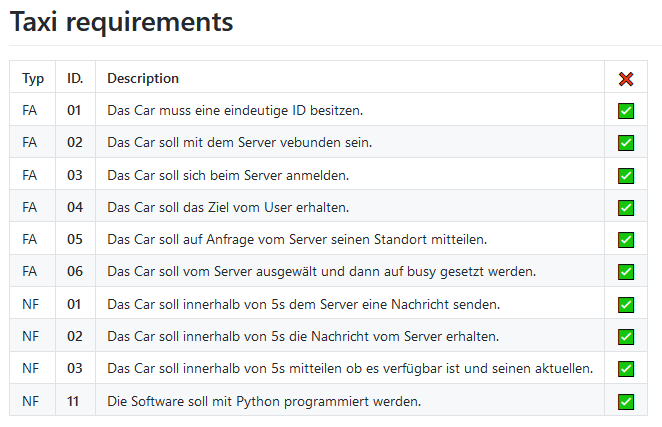
\includegraphics[width=0.48\textwidth]{Bsp_requirments.png}
     \caption{Requirments}
\end{figure}

\subsection{Use-Case}

Der Nächste Schritt im Projekt, ist aus dem gesammelten Informationen der Requirements, Use-Case Diagramme für jeden Client zu erstellen.
Use-Case Diagramme verdeutlichen die Aufgaben und Verbindungen zwischen den einzelnen Clients.

Vorab Registrieren sich alle Clients beim Server, so ist der Server mit jedem Client verbunden. Nun bekommt der Server eine Message vom User, 'request car'.

Folgend wird 'select closest car' vom Server durchgeführt und dem nächsten gelegenen Car mitgeteilt, das eine anfragende vom User eingegangen ist. Zudem sind in der Message die Koordinaten des Users enthalten, woraufhin das Car zu diesem Standort fährt.

Der Server setzt das bestellte Car auf Busy, 'change car status'.
Danach erhält das Car eine Message vom User mit dem gewünschten Zielort und bringt ihn dort hin. Am Zielort setzt der User dann das Car beim Server wieder auf free. Zum Schluss erfragt der Server den neuen Standort des Cars und schließt die Handlung damit ab.


\begin{figure}[htbp] 
  \centering
     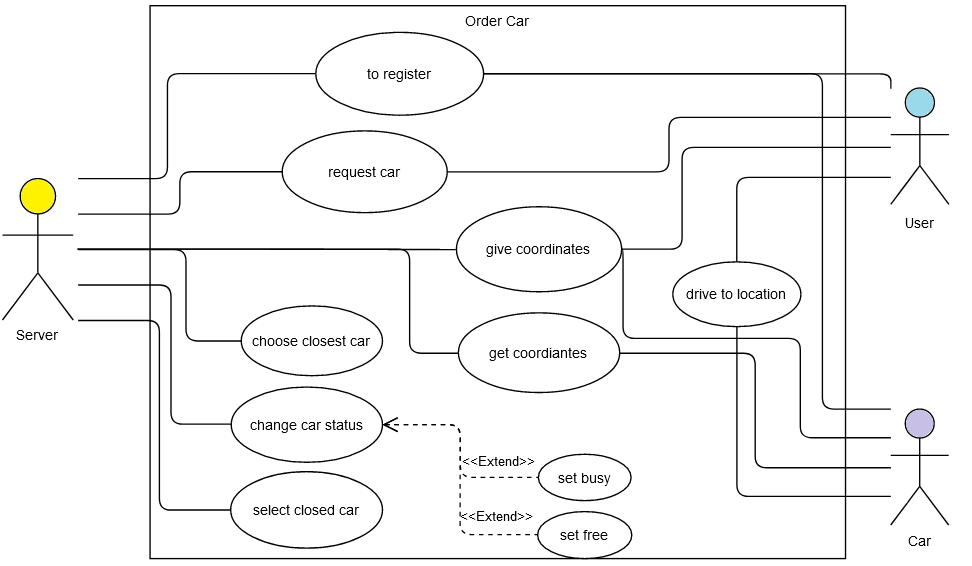
\includegraphics[width=0.48\textwidth]{Use-Case_Server.png}
     \caption{Use-Case}
\end{figure}

\subsection{Klassendiagramm}


\begin{figure}[htbp] 
  \centering
     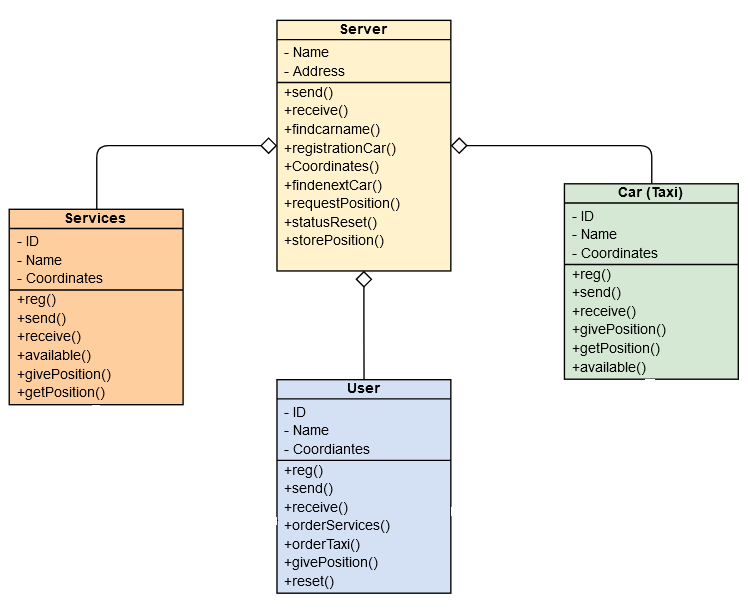
\includegraphics[width=0.48\textwidth]{Class_diagramm.png}
     \caption{Use-Case}
\end{figure}

\section{MQTT}
Das \textbf{Message Queuing Telemetry Transport}, oder kurz \textbf{MQTT}, ist ein Protokoll, welches für die Kommunikation zwischen Maschinen bestimmt ist. Somit eignet sich dieses Protokoll auch im Wesentlichen für seinen Einsatz im Anwendungsbereich der Automatisierung und ganz besonders im Bereich des Internet der Dinge (\textbf{IoT} Internet of Things). Da aufgrund seines Aufbaus Geräte mit wenig Akkukapazität so gut wie keine eigene Rechenleistung erbringen müssen, um Nachrichten zu empfangen oder senden zu können, ist vor allem bei Akku-betriebenen Geräten ein Vorteil zu erkennen.\\
Erreicht wird dies durch den generellen Aufbau des Protokolls mittels Subscriber/ Publishern und einem zentralen Broker, wobei der Broker der verwaltende und Daten haltende Part ist und einem Server nahe kommt. Zudem gibt es die Subscriber, die Nachrichten empfangen können- ein Beispiel hierfür wären Aktoren. Die Publisher hingegen kommen zum Beispiel als Sensoren zum Einsatz, sie teilen der Netzwerkstruktur ihre Informationen mit. Die Einordnung als Subscriber oder als Publisher ist aber in keinem Fall exklusiv, sodass Geräte auch in einem hybriden Modus sowohl versenden als auch empfangen können, das wäre zum Beispiel bei einem Smart Home-Server der Fall.\\
 Ein ganz wesentlicher Vorteil des MQTT-Protokolls liegt in seiner Struktur als Publishing and Subcribe Verfahren. Dadurch, dass das Senden der Nachrichten nicht als Direktverbindung der Clients untereinander, sondern mit dem Umweg über den Broker geschieht, sind die Geräte in der Lage, Nachrichten sicher zu empfangen, auch wenn sie gerade nicht auf Nachrichten-Empfang stehen.\cite{b1}
 \begin{figure}[h]
 \caption{MQTT-Struktur \cite{b1}}
 \centering
 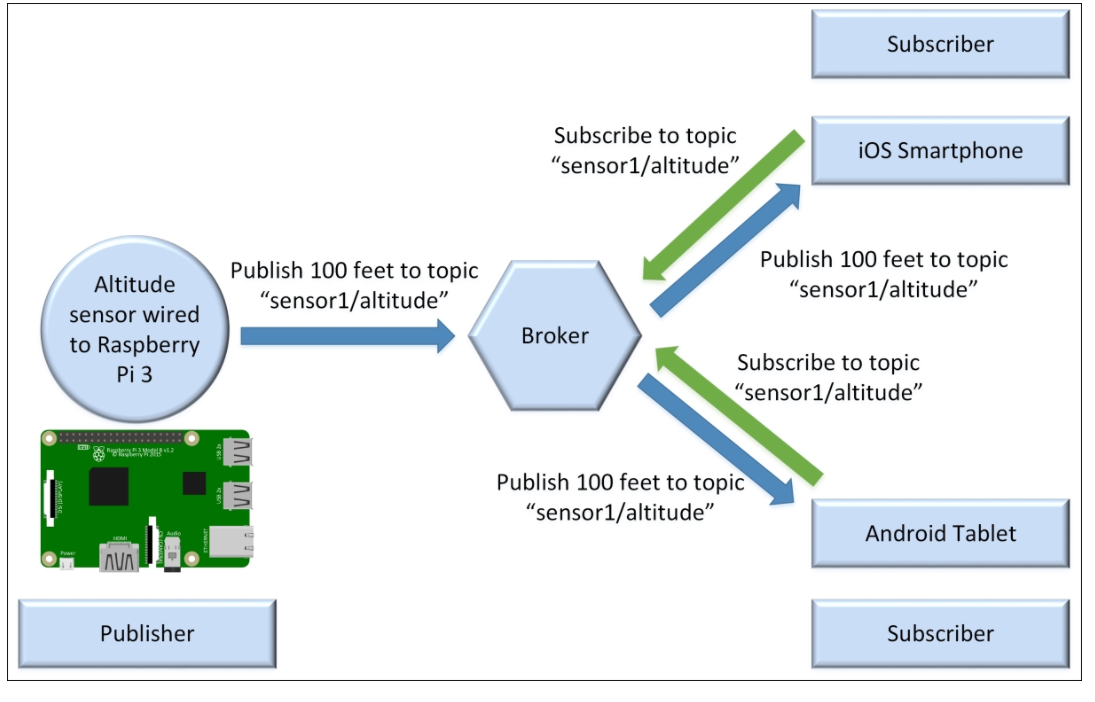
\includegraphics[scale=0.4]{mqtt_structure}
 \end{figure}
Jedoch bringt dieses Verfahren auch einen gravierenden Nachteil mit sich. Aufgrund dessen, dass Nachrichten nicht in einer eins-zu-eins-Übertragung miteinander geteilt werden, müssen Nachrichten auf eine andere Art und Weise zu ihrem Ziel gelangen. Fatal wäre hier zu glauben, auf eine Zuordnung der Nachrichten verzichten zu können. Da gerade in einem Smart Home viele ähnliche Geräte verbaut werden und somit auch viele ähnliche Werte versendet werden, wäre eine einfache Zuordnung nun nicht mehr ohne weiteres möglich.
Abhilfe schafft im MQTT-Protokoll ein Nachrichtenfilter mit einer Art Kanäle, die die Geräte "abonnieren" können, um nur relevante Daten zu erhalten\cite{b1}. Diese Kanäle haben Ähnlichkeit mit Adressen, geben Filter und Subfilter für die Nachrichtenverteilung an und werden nach dem Schema: \textsf{Erdgeschoss/Rolladensteuerung/Fenster1/Motor} erstellt, um ein Beispiel für die Ansteuerung des 1. Fensters im Erdgeschoss zu nennen. \\
Vorteile bietet MQTT des weiteren dank der Möglichkeit, das IP-Protokoll und somit TCP und TLS zu verwenden, was der Nachrichtenübertragung einen gewissen Schutz gegen das Verlieren von Nachrichten bietet, was gerade in kritischen Systembereichen einen Mehrwert hat. Und dank der Verschlüsselung mittels TLS bietet es einen Schutz gegen das zugreifen von unbefugten.



\section{Warum haben wir was benutzt? (Programmiersprache/ Umgebung, Github)}
Bevor wir angefangen haben das Projekt durchzuführen und zu implementieren haben wir uns überlegt, welche Programmiersprache, welche Programmierumgebung und welche Plattform wir zur Versionsverwaltung benutzen wollen.

\subsection{Python}
MQTT kann mit verschiedensten Programmiersprachen, wie Java, C++ oder Python programmiert werden.
Die Sprachen haben ihre eigenen Vor und Nachteile, wodurch sie besser oder nicht so gut geeignet sind.
Java und C++ sind statisch typisiert und kompilierte Sprachen, was diese zur Laufzeit schneller macht. Der Code muss aber auf unterschiedlichen Betriebssystemen neu Kompiliert werden, da das Programm sonst nicht funktioniert. https://www.bmc.com/blogs/python-vs-java/
https://www.bitdegree.org/tutorials/python-vs-c-plus-plus/

Auf der anderen Seite gilt bei Python „write once, run anywhere“ was bedeutet, dass der geschriebene Code auf allen Betriebssystemen funktioniert. 
Außerdem ist Python einfacher in der Verwendung und einfacher zu verstehen. Weiter sind im Vergleich zu Java oder C++ die Codezeilen kürzer.
Wir haben uns für Python endschieden, weil der Code auf allen Betriebssysteme einfach ausgeführt werden kann. Ein weiterer Grund ist, dass Python einfacher in der Verwendung ist.


\subsection{Atom}
Um in Python zu programmieren haben wir das Programm Atom benutzt. Dieses ist einfach zu bedienen und der Code kann über F5 direkt getestet/ausgeführt werden.
Es wird eine Datei mit der Endung .py erstellt und schon kann mit der Programmierung begonnen werden.

\subsection{Github}
Um das Projekt zu Organisieren und auf dem aktuellen Stand zu halten haben wir Github verwendet.
Über Github ist der gesamte Programmcode und die Githistorie auf jedem Entwicklercomputer verfügbar, wodurch einfaches Zusammenfügen der Code Abschnitte  ermöglicht wird.
https://kinsta.com/de/wissensdatenbank/was-ist-github/
\section{ServicesCode}
In diesem Abschnitt wird der Teil Services beschrieben. 
Die Aufgabe der Services war es, das sich verschiedene Servicefahrzeuge, wie Police, Firefighter und Ambulance über den Server anmelden können. Eine weitere Aufgabe war es das die Servicefahrzeuge auf Anfrage den User abholen und zu einem Zielort bringen.
So wird über die Methode registration ein Service Fahrzeug (hier: Police) angemeldet. Wenn in id: register steht wird eine id vom Server zugewiesen.
Damit das fahrzeug eine Startkoordinate zugeordnet wird, wird in der Methode policecoor eine Zufällige Koordinate generiert. 
\newline
\textit{registrierung Servicefahrzeug}
\begin{lstlisting}
def policecoor(): 
    zahly = randint(0, 4)
    zahlx = randint(0, 4)
    return str(zahly)+";"+str(zahlx)

def registration():
    global coor
    global name
    coor = policecoor()

    data = {
    "id": "register",
    "name": name,
    "coordinates": coor #Requirement: FA4
    }
    send("hshl/mqtt_exercise/services/police", json.dumps(data)) #Requirement: FA2; Requirement: FA3
\end{lstlisting}

Wenn ein Servicefahrzeug angefordert wird bekommt es den Standort des Users zugeschickt. 
Das Fahrzeug fährt dann zu den vom User erhaltene Koordinaten und setzt seine Koordinaten auf den Standort des Users.


\textit{Zum User fahren}
\begin{lstlisting}
def drivetoUser(usercoor):
    print("New destination: "+usercoor) #textausgabe
    coor = usercoor   #setzen der pickup koorindanten zu dem standkoordinaten
    time.sleep(1)#warten
    print("Arrival at: "+usercoor) #textausgabe
\end{lstlisting}


Der neue Standort wird in einer jason Datei mit der zugewiesen id und einer msg: Arrival in einem Dataset gespeichert.
\begin{lstlisting}
        data = {
        "id":id,
        "msg": "Arrival",
        "coordinates": js['coordinates']
        }
\end{lstlisting}
Wenn das Fahrzeug beim User angekommen ist, wird es auf bussy (Fahrzeug ist unterwegs) gesetzt.


Als nächstes bekommt das Fahrzeug eine Zielkoordinate vom User mit dem jeweiligen Usernamen.
Über die Methode userDestination wird der User zum Zielort gefahren. Der neue Standort ist dann die Zielkoordinate (destinationcoor).


\textit{Zum Zielort fahren}
\begin{lstlisting}
def userDestination(destinationcoor, guestname):
    print("New destination, drive "+guestname+" to: "+destinationcoor) #textausgabe
    coor = destinationcoor #setzen der zielkoordinaten in den standort des fahrzeugs
    time.sleep(1) #schlafen eine sekunde
    print("Arrival at: "+destinationcoor)
\end{lstlisting}

Dies wird in einem Dataset mit der id des Fahrzeugs, der msg: Arrival at destination und der destinationcoor gespeichert.

\begin{lstlisting}
        data ={
        "id":id,
        "msg": "Arrival at destination",
        "coordinates": js['destination']
        }
\end{lstlisting}
Der User setzt das Fahrzeug wieder auf free (Fahrzeug bereit für neue Anfragen).


Zuletzt sendet das Fahrzeug auf Anfrage des Servers seinen aktuellen Standort mit seiner id und dem Namen des Fahrzeugs. 
\textit{übergabe der neuen Koordinaten}
\begin{lstlisting}
        data={
        "id":id,
        "name":name,
        "coordinates":coor
        }
        send(json.dumps(data),"hshl/mqtt_exercise/set_position")

\end{lstlisting}





















\section{User Code}\label{usercode}
Der Code des Users wurde hinsichtlich der Anforderungen so gestaltet, dass dieser dem Nutzer sowohl eine ID als auch einen Nutzernamen zuweist. Darüber hinaus werden dem Server für die Weiterverarbeitung auch die aktuellen Koordinaten der Person übergeben. Im Folgenden wird der in diesem Projekt durch Python realisierte Code, in Abschnitte unterteilt und kurz in seiner Funktion erläutert.\\
\\
Im ersten Schritt nach Programmstart wird der User gebeten sich mit dem Befehl \textit{reg} in der Eingabeaufforderung anzumelden. Daraufhin bekommt dieser seine ID, sowie seinen Nutzernamen und Standort übergeben und im Server hinterlegt. Den entsprechenden Ausschnitt des Codes ist im folgenden zu sehen.

\begin{lstlisting}
#Login des Users
def userin(userinput):
    if userinput =="reg":
        getid()
        receive()
        pass
\end{lstlisting}

Gleiches gilt für die anschließende Bestellung eines der Services. Der Nutzer ist über den Eingabebefehl \textit{order(geforderter Service)} in der Lage den geforderten Service zu rufen. Hierbei stehen folgende Fahrzeugtypen zur Auswahl.

\begin{itemize}

	\item taxi
	\item police
	\item ambulance
	\item firefighter

\end{itemize}

Die damit aufgerufene Methode, in diesem Beispiel für das Taxi, \textit{def ordertaxi()} übergibt die damit zusammenhängenden Daten des Users, mittels des Aufrufs \textit{send(…)} an den Server.
Hier ist die Klasse des Taxis in der Lage sich die notwendigen Informationen auszulesen.

\begin{lstlisting}
#Call For Taxi
def ordertaxi():
    global id
    global cartype
    data1 = {
        "type": "taxi",
        "id": id,
        "coordinates": coordinates
        }
    cartype = "taxi"
    time.sleep(5)
    send(json.dumps(data1),"hshl/mqtt_exercise/user/"+str(id))
\end{lstlisting}

In den weiteren Schritten wird der User direkt mit dem Taxi verbunden um miteinander zu kommunizieren. Dies entlastet zum einen den Server und hat zum anderen den Vorteil die Ausführungszeiten zu verringern. Das Taxi wird sich mitteilen sobald es den Nutzer erreicht hat und dieser wiederum ein weiteres Paar Koordinaten als sein Ziel angeben. Nach erreichen der vom User geforderten Position kann das Servicefahrzeug von eben diesem wieder als \textit{free} gesetzt werden und kann sich um weitere Aufträge anderer Nutzer kümmern.

\begin{lstlisting}
#Seting Vehicle Status To Free
def setToFree():
    global id
    global idCar
    global cartype
    print("SERVICE VEHICLE SET TO FREE")
    data = {
    "type": cartype,
    "id": id,
    "idCar": idCar,
    }
    send(json.dumps(data),"hshl/mqtt_exercise/user/"+str(id)+"/status/reset")
\end{lstlisting}


\section{TaxiCode}

Die Aufgabe des Taxis ist es über den MQTT Server mit dem Server und dem User zu kommunizieren.
 
Über die erhaltenen Messages fährt das Taxi zum User und bringt ihn zu seinem Zielort.

Der erste Schritt vom Taxi ist, sich beim Server mit seinem Namen zu registrieren. 

Folgend weißt der Server dann dem Taxi seine ID zu.

\begin{lstlisting} 

data = {
	"id": "register", 
	"name": name,
	"coordinates": coor
    }
    
\end{lstlisting}



Daraufhin erhält das Taxi eine Message vom Server, dass ein User ein Taxi bestellt hat. 
Nun liest das Taxi die Koordinaten vom User aus. 

\begin{lstlisting} 
        data = {
        "id":id,
        "msg": "Arrival",
        "coordinates": js['coordinates']
        }
\end{lstlisting}



Mit den erhaltenden Koordinaten, weiß das Taxi an welcher Stelle sich der User befindet und fährt zu seiner aktuellen Position.
Am Zielort angekommen, wartet das Taxi auf die neue Message vom User, mit seinem neuen Zielort.


\begin{lstlisting} 
        data ={
        "id":id,
        "msg": "Arrival at destination",
        "coordinates": js['destination']
        }
\end{lstlisting}



Zum Schluss erhält das Taxi eine Anfrage vom Server, mit seiner neuen Position und sendet diese dann zum Server.

\begin{lstlisting} 
data={
        "id":id,
        "name":name,
        "coordinates":coor
        }
        send(json.dumps(data),
        "hshl/mqtt_exercise/set_position")

\end{lstlisting}

\section{Server}
In diesem Kontext spielt der Server eine sehr wichtige Rolle in der Kommunikation zwischen den ausführenden Parts des Projektes. Durch den Server und seine Strukturen wird letztendlich erst eine Plattform geschaffen, die allen Fahrzeugen und den Kunden (Usern) eine Möglichkeit bietet, eine Verbindung untereinander zu schaffen und weitere Aufgaben zu erledigen. Konkret waren die Aufgaben des Servers:
\begin{table}[h]
\begin{tabular}{lcr}
Anmeldung von Clients\\
Das nächstgelegene Fahrzeug finden\\
Jedem Client eine eindeutige ID zuordnen\\
Übermittlung der Fahrzeugdaten an den Kunden\\
Interne Verarbeitung einer Fahrzeugbestellung\\
\end{tabular}
\end{table}
\subsection{Anmeldung von Clients}
Aufgabe des Servers ist es, eine Anmeldung von Clients zu ermöglichen, um einerseits nur aus dem Pool der aktuell aktiven, freien Fahrzeuge auszuwählen und andererseits, einer unbekannten Menge an Fahrzeugen und Kunden die Möglichkeit zu bieten, am Angebot teilzuhaben. Zu den Clients gehören sowohl die Kunden (User), wie auch alle Fahrzeugtypen. Damit sind alle Servicefahrzeuge mit den Unterkategorien: Police, Firefighter, Ambulance gemeint und zuletzt auch Fahrzeuge der Kategorie Taxi.\\
Um auf eine unbekannte Anzahl an sich zu registrierenden Clients reagieren zu können, muss der initiative Schritt durch den Client erfolgen. Zur Registrierung sendet der Client eine Nachricht mittels MQTT-Protokoll über die Adressen des Users oder der Fahrzeugtypen mit dem ersten Teil \textsf{"adresse = hshl/mqtt\_exercise/"} und der Endung des jeweiligen Fahrzeugtypen, also: \textsf{"user,taxi,police,firefighter,ambulance"} an den Server. Dieser verarbeitet die Nachricht bei Erhalt in der Funktion
\begin{lstlisting}
def receive()
	....
	messageprocessing(temp)
	....
\end{lstlisting}
 wobei die Aufgabe der Funktion \textit{receive()} eher die generelle Verarbeitung der MQTT-Nachricht darstellt und nicht die Zuordnung der Nachricht zu einen bestimmten Anwendungszweck.
Dieser wird anschließend durch den Aufruf der Funktion \textit{messageprocessing} und eine Teilung des übergebenen Arrays in die Informationen zu Inhalt und Adresse der Nachricht erreicht.
Um ein Auslesen der Nachricht überhaupt zu ermöglichen ist es notwending, die empfangene Nachricht erst in das Json-Format zu codieren, um anschließend die Vorteile einer Verarbeitung mit Json-Datasets zu nutzen. Dies wird mit der Textzeitle \begin{lstlisting}
def messageprocessing(msg)
	json.loads(str(msg[1]))
\end{lstlisting}
 erreicht.\\
 Zur besseren Identifizierung und Klassifizierung als Registrierungs-Nachricht, wird in dieser die ID des Clients durch das Wort "register" ersetzt. Dies dient- wie schon erwähnt- einerseits der besseren Einordnung und andererseits half das Lesbar-Halten von Nachrichten für Menschen bei der Entwicklung ungemein. Einen negativen Einfluss auf den erfolgreichen Ablauf der Registrierung des Clients hat dies nicht, da eine ID erst mit Antwort des Servers an den Client vergeben wird. Die Nachricht, die ein Client zur Registrierung/Anmeldung senden muss, sieht wie folgt aus:
\begin{lstlisting}
    data={
    "id": "register",
    "name": name,
    "coordinates":coor
    }
\end{lstlisting}
Zudem wird in der internen Verarbeitung ein neuer Kanal für die weitere Kommunikation mit dem Client geschaffen, sodass eine direkte Kommunikation mit diesem möglich ist, ohne dass andere Clients hierdurch beeinträchtigt werden. Die Adresse des neuen Kanals wird unter Zuhilfenahme  der durch den Server in den Funktionen \textit{regestrationUser(data)} und \textit{registrationCar(data, type)} vergebenen ID geöffnet und mittels einer Nachricht auf dem Kanal \textsf{"hshl/mqtt\_exercise/user/back"} an diesen zurück gesendet. \\
Anhand des Quellcodes für das Registrieren des Users wird gezeigt, wie die Vergabe einer neuen ID und das Einspeichern des Clients in den Server funktioniert. Dies ist ganz ähnlich für das Vorgeben bei der Registrierung von Fahrzeugen mit dem einzigen Unterschied, dass in diesem Fall mittels einer Separierung durch den Übergabewert "type" die einzelnen Fahrzeuge unterschieden werden können. Des weiteren wird bei der Registrierung der Fahrzeuge noch der Status "free" vergeben.\\
Zuerst wird durch den Aufruf der Funktion \textit{findid(user)} die kleinste noch freie ID aus der Liste der angemeldeten Fahrzeuge gesucht, indem die höchste vergebene ID gesucht wird und um einen Zähler höher zurückgegeben wird. Anschließend wird in der Methode \textit{registrationUser(data)} durch ein weiteres Durchlaufen der Liste geprüft, ob bereits ein User mit demselben Namen vorhanden ist und bei negativem Ergebnis in die Liste aller User eingetragen.\\ Der User bekommt abschließend auf dem Rückkanal eine Nachricht mit seiner eindeutigen ID.
\subsection{Bestellen eines Fahrzeugs}
Nach erfolgreicher Registrierung ist es für den Kunden möglich, Fahrzeuge zu bestellen und für Fahrzeuge ist es möglich, durch einen Kunden bestellt zu werden. In diesem Fall spielt nun der Server eine verbindende Rolle, indem er eine Anfrage des Kunden entgegennehmen kann und diese an ein von ihm ausgewähltes Fahrzeug weiterleitet. Die Wahl des passenden Fahrzeugs trifft hierbei der Server, da nur er die Positionen aller Teilnehmer kennt und somit das nächstgelegene Fahrzeug auswählen kann.\\
Eine Anfrage durch einen Kunden wird unter dem im Vorfeld bei der Regestrierung neu geöffneten Kanal in Verbindung mit der ID des Kunden und einer Nachricht mit einem Inhalt, der Informationen über den Kunden, den Koordinaten des Kunden und dem gewünschten Fahrzeugtyp, gestartet. Beispielsweise kann durch den Kunden $ID: 0, Name: Peter, Koordinaten: 2,4$ unter der $Adresse=\textsf{hshl/mqtt\_exercise/user/[ID] }$ mit folgender Nachricht ein Taxi bestellt werden \begin{lstlisting}
data = {
	"type": "taxi",
    "id": id,
    "coordinates": coordinates
    }
\end{lstlisting}
Intern verarbeitet der Server die Anfrage des Kunden zuerst, indem er aus dem Type die richtige Liste an die Funktion \textit{findnextcar(gpsUser, car)} übergibt, die das nächstgelegene Fahrzeug des Typs Taxi durch die Koordinaten, die durch den Kunden übermittelt wurden, findet.\\
Nach erfolgreicher Ermittlung des nächstgelegenen Fahrzeugs wird dem Kunden der Datensatz des Fahrzeugs auf dem Kanal \textsf{hshl/mqtt\_exercise/user/"id"/order/back} , wobei "id"  die kundenspezifische ID des Antragstellers darstellt und somit nur der Kunde Antwort erhält, der in diesem Moment auch ein Fahrzeug bestellt hat. Als weiteren wichtigen Schritt ist Sorge dafür zu tragen, dass die Einhaltung der Anforderung \textbf{F-S02} durch die Anwendung von \textbf{F-S08} nicht verletzt wird und nur Fahrzeuge vergeben werden, die den Status "free" besitzen. Das wird erreicht indem der Status eines freien Fahrzeugs durch den Status "busy" ersetzt wird, wenn er an einen Kunden verschickt wird.
\subsubsection{Finde das nächstgelegene Fahrzeug}
Um das Fahrzeug  zu finden, das dem Kunden am nächsten gelegen ist, muss zuerst die vorhandene Karte abgebildet werden können. Dies wird erreicht indem Planquadrate eingezeichnet werden. Durch die festgelegten Planquadrate lässt sich anschließend durch Iterieren der Planquadrate und Abgleichen der Liste der Fahrzeuge das gesuchte Fahrzeug finden. So in der vereinfachten Theorie, allerdings entstehen bei der Umschlüsselung auf den konkreten Fall diverse Probleme, die das Finden des nächstgelegenen Fahrzeug und nicht irgendeines Fahrzeugs komplizierter gestalten als zu Anfang angenommen.\\
dDurch den Umstand, dass der Mittelpunkt der Suche bedingt durch den variablen Standort des Kunden nicht zwingend der Mittelpunkt der Karte darstellen muss, kam als optimale Lösung ein Ring-artiges Erweitern der Suche um den Standort des Kunden infrage. Dieses wurde mittels Schleifeniteration geschaffen.\\
Die erste Schleife mit der Laufvariable "k" gib an, um welchen Ring um den aktuellen Standort des Kunden es sich handelt. Die zweite Schleife steht für die y-Achse der Karte und gibt somit die Reihen der Quadrate an. Sie iteriert von einem Startpunkt an, der sich auszeichnet durch die Gegenzahl von der Ringstufe $k$ minus einem Zähler $i_{starpunkt} = (k-1)*(-1)$ bis zu dem Endpunkt der durch k plus einem Zähler beschrieben werden kann $i_{endpunkt} = k+1$. Die x-Achse wird durch einen weiteren Schleifendurchlauf abgebildet und spiegelt die Spalten der Karte wider. Die x-Achsen-Schleife läuft vom Startpunkt $j_{starpunkt} = i $, also der linken oberen Ecke des aktuellen Rings, bis zum Endpunkt $j_{endpunkt} = k+1$, also der rechten unteren Ecke des aktuellen Rings. Eine letzte Schleife vergleicht letztendlich die angegebene Position mit der Liste der angemeldeten Fahrzeuge ab, um zu prüfen, ob sich an der aktuellen Koordinate ein Fahrzeug befindet.
\begin{lstlisting}
def findnextCar(gpsUser,car):
    cancle = 0
    for k in range(int(gpsUser.split(";")[0]),5):
        for i in range((k-1)*(-1), k+1):
            print("i ist:"+str(i))
            for j in range(i, k+1):

                print("j ist:"+str(j))
                for c in range(0,len(car)):
                    print("search for car: "
                    		+ str(car[c]))
...
\end{lstlisting}
Ein Nachteil den der beschriebene Code innehat ist allerdings, dass bei jedem Durchlauf nur um einen Ring erweitert wird. In Wirklichkeit wird hingegen nicht ein Ring geprüft, sondern ein Quadrat jedes mal um einen Ring erweitert. Dies hat zum Nachteil, dass bei jedem Durchlauf auch jedes mal bereits geprüfte Felder ein weiteres mal geprüft werden, was einen deutlich hemmenden Einfluss auf die Laufzeit des Programmes hat und letztendlich auch ein überflüssiges Unterfangen ist. Demnach ist bei einer möglichen Optimierung darauf zu achten, bereits geprüfte Felder nicht ein weiteres Mal zu überprüfen. Eine mögliche Umsetzung wäre, die vorhandenen Schleifen für die x- Achse  und die y- Achse in jeweils zwei Schleifen aufzuspalten, wobei in diesem Fall die erste Schleife den negativen Bereich auf der linken und oberen Seite des Standortes prüfen würde und die zweite Schleife den rechten und unteren positiven Bereich der Karte.
\begin{figure}[h]
\caption{Optimierung Schleifendurchlauf findnextcar()}
\centering
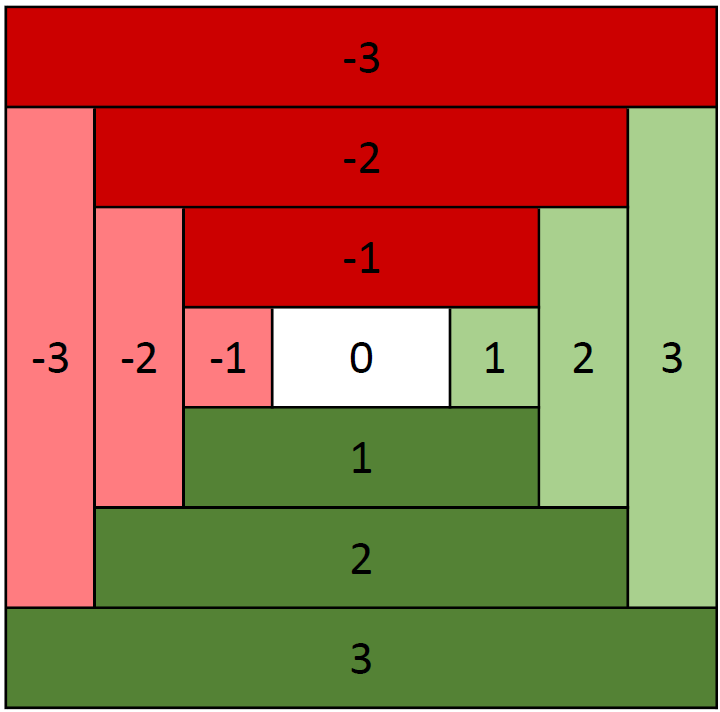
\includegraphics[scale=0.5]{opti_findnextcar}
\end{figure}
Anschließend wird als letzter Schritt innerhalb der letzten Schleife noch abgeglichen, ob sich ein freies Fahrzeug mit den passenden Koordinaten auf der entsprechenden aktuell geprüften Position befindet, beispielhaft dargestellt für den Bereich $-y,+x = \{-,+\}$. Aus der Tabelle \ref{tab.1} kann in Verbindung mit den aktuellen Schleifen-Variablen die aktuell zu prüfende Position bestimmt werden, wie in Beispiel Positionsabgleich zu sehen. Zudem wird noch sicherheitshalber ein Counter erstellt, der einen exit nach drei Durchläufen ohne Ergebnis ermöglicht.
\begin{lstlisting}
#Bespiel Positions-Abgleich#
...
elif int(car[c][2].split(";")[0]) == -i
and int(car[c][2].split(";")[1]) == j:
	if car[c][3]== "free":#Requirements: F-S11
    	return car[c]
    else:
        c=c-1
       	cancle = cancle+1
\end{lstlisting}
\begin{table}[h]
\centering
\label{tab.1}
\caption{Abgleich-Tabelle für die Positionsbestimmung der Fahrzeuge}
\begin{tabular}{lcccccr}
--,--&--,-&--,=&--,+&--,++\\
-,--&-,-&-,=&-,+&-,++\\
=,--&=,-&=,=&=,+&=,++\\
+,--&+,-&+,=&+,+&+,++\\
++,--&++,-&++,=&++,+&++,++\\
\end{tabular}
\end{table}
Als Rückgabewert wird der Datensatz des Fahrzeugs, das dem Kunden am nächsten liegt, an den Aufruf zurück gegeben. Dieser kann anschließend an den Kunden übermittelt werden.
\subsection{Ankunft am Ziel}
Für den Server ist durch die Vermittlung des nächstgelegenen Fahrzeugs an den Kunden der Hauptteil seiner Aufgabe erledigt und das Primärziel erreicht. Demnach wurde dem Kunden auf effiziente Weise ein Fahrzeug vermittelt und im Falle einer Buchung eines Service-Fahrzeugs im Optimalfall sogar Leben gerettet. Allerdings stehen nicht unbegrenzt Fahrzeug-Ressourcen zur Verfügung, weswegen eine einfache Nutzung dieser im realen Umfeld logischerweise niemals Anwendung finden würde. Deswegen ist es zwingend erforderlich, eine Möglichkeit zu bieten, Fahrzeuge fortlaufend an Kunden zu vermitteln.\\
Da aufgrund der zu Beginn des Projektes beschriebenen Systemumgebung der Server seinen Einfluss an den georderten Fahrzeug mit der Übermittlung der Fahrzeugdaten zum Kunden an diesen die Kontroll-Gewalt abgibt \cite[?], ist es dem Server erst durch Initiative des Kunden möglich, Fahrzeuge wieder in den Status "free" zu nehmen. Dieses Verfahren bietet auf eine erste logische Betrachtung die Vorteile, dass solange der Kunde nicht aussteigt, ein Fahrzeug auf keinen Fall frei werden kann. Dies kommt der Praxis sehr nahe und bildet deswegen sehr gut die Realität ab. Ein Nachteil für dieses Vorgehen ist allerdings, dass durch die Abgabe der Kontroll-Gewalt der Server keinen Einfluss mehr auf das Fahrzeug hat, solange es nicht durch die Nachricht des Kunden freigegeben wird. Sollte nun der Kunde aussteigen und   keine Nachricht an den Server senden, oder sollte diese verloren gehen, so wird dieses Fahrzeug auf unbegrenzte Zeit als belegt verbucht bleiben und somit nicht genutzt werden können. \\ Eine Lösung des Problems wäre ein Timer, der nach einer bestimmten Zeit eine Anfrage an jedes belegte Fahrzeug sendet, ob dies immer noch durch den Kunden belegt ist. Des Weiteren könnte eine Rückanmeldung eines Fahrzeugs auch auf Nachricht des Fahrzeugs umgesetzt werden, sodass das Fahrzeug sich in dem Moment des Freiwerdens beim Server zurück anmeldet.
Allerdings würde der verwendete Kerncode auch in beiden Optimierungsfällen ähnliche Funktionen aufweisen.
\\
Eine Nachricht zur Freigabe eines Fahrzeugs wird mittels einer Nachricht über den Kanal \textsf{"hshl/mqtt\_exercise/user/"id"/status/reset"} und dem Inhalt "type" , "id" des Users und der id des Fahrzeugs "idCar" an den Server gesendet. Dieser ist nun in der Lage durch den Aufruf der Funktion \textit{$statusReset(int(js["idCar"]),str(js["type"]))$} mittels Fahrzeugtyp und dessen ID, dem benutzten Fahrzeug wieder den Status "free" zuzuordnen, ein weiterer wichtiger Schritt wird mittels Funktionsaufruf
\textit{$requestPosition(js["idCar"],js["type"],\\str(findcarname(js["idCar"],str(js["type"]))))$}
vollzogen. Angefragt wird der aktuelle Standort des freigegebenen Fahrzeugs, um in fortlaufenden Buchungen wieder die Möglichkeit zu bieten, dem Kunden sein nächstgelegenes Fahrzeug zu Verfügung zu stellen. Demnach sendet der Server dem gerade freigegebenen Fahrzeug über den Kanal \textsf{"hshl/mqtt\_exercise/get\_position"} eine Anfrage mit dem Inhalt "id" des Fahrzeugs und dem dazugehörigen Namen und erhält im besten Fall eine Antwort über den Kanal \textsf{"hshl/mqtt\_exercise/set\_position} mit Informationen über "id" des Fahrzeugs, seines "typs" und zuletzt der aktuellen "coordinates". Diese Informationen werden dann in der passenden Liste des Typs für das aktuelle Fahrzeug aktualisiert.
\begin{lstlisting}
    data = {
    "type": cartype,
    "id": id,
    "idCar": idCar,
    }
\end{lstlisting}
\subsection{Periodische Abfrage der Fahrzeugposition}
In der Realität stehen Fahrzeuge wie Taxen oder Polizeifahrzeuge selten still. Aus diesem Grund ist die Wahrscheinlichkeit ziemlich hoch, dass diese Fahrzeuge nach ihrer Anmeldung im Laufe der Zeit ihre Position verändern. Deswegen erscheint es nur sinnvoll, in regelmäßigen Abständen deren Position zu kontrollieren- beziehungsweise abzufragen- um immer zu garantieren, dass das nächst gelegene Fahrzeug ausgewählt werden kann.\\ Problematisch ist hierbei, dass die Menge an zu überprüfenden Fahrzeugen einen erheblichen Zeitaufwand in Anspruch nimmt und somit nicht so schnell wie möglich auf Anfragen eines Clients reagiert werden kann, oder im schlimmsten Fall sogar Nachrichten verloren gehen können. Aufgrund dessen ist es notwendig, die Abläufe von Nachrichtenverarbeitung und -abfrage der Position voneinander zu trennen. Genutzt wurde hierfür die Möglichkeit, mittels Python Erweiterung \textbf{threading} auf Multi-Threading zu setzen und somit die Aufgaben in zwei verschiedenen Prozessen aufzusplitten. Dies hat zwar zur Folge, dass die Auslastung des ausführenden Systems ein wenig höher ist, allerdings sind selbst Einplatinen-Computer schon seit Längerem mit Mehrkern-Prozessoren ausgestattet, was jegliches bedenken bezüglich der Auslastung ihm Rahmen dieses Projektes hinfällig macht.

\section{Fazit}
Das Ziel dieses Projekts bestand darin ein Programm zu entwickeln, welches dazu dient eine Person (hier auch User oder Nutzer) mithilfe einfachster Schritte einen speziellen Service in Anspruch nehmen zu lassen, welche sich aus dem vorherigen Kapitel unter dem Begriff Servicefahrzeuge entnehme lassen. Hierbei wurden diverse Anforderungen schon vorher festgelegt und definierten den Projektrahmen. So wurde gefordert, dass jeder Nutzer dieser Anwendung, mittels einer eigenen ID identifiziert werden kann und zudem seinen Namen und seine aktuellen Koordinaten an den Server schickt. Der Server wiederum diente der Verarbeitung und Speicherung der erhaltenen Nachrichten, um so eine Art 'Schwarzes Brett' für alle Services darzustellen. Die Servicefahrzeuge waren somit in der Lage sich die nötigen Informationen zu holen und mit dem Nutzer in Kontakt zu treten.\\
Im Bezug auf die Zukunft und die mögliche Anwendbarkeit einer solchen Anwendung lässt sich bisher nur spekulieren. Für einfache Services wie Taxen, welches ebenfalls eine Dienstleistung in dieser Anwendung ist, ist diese Art von Technik bereits durch ein namhaftes Unternehmen weltweit vertreten. Hinsichtlich der zur Verfügung Stellung von Polizei, Krankenwagen und Feuerwehr müssen jedoch noch viele Ressourcen in ein flächendeckendes und einheitliches System gesteckt und unter Berücksichtigung der Sicherheit beurteilt werden.\\
In diesem Fall war das Projekt jedoch ein Erfolg und könnte die Basis für ein eben solches System darlegen. Durch die gute Koordinierung und Rücksprache ließen sich Probleme und Anregungen schnell besprechen und in der Gruppe lösen.






\begin{thebibliography}{00}
\bibitem{b1}  Gastón C. Hillar, MQTT essentials, a lightweight IoT protocol : the preferred IoT publish-subscribe lightweight messaging protocol, Packt Publishing, Birmingham, United Kingdom, 2017
\bibitem{b2}  https://www.bmc.com/blogs/python-vs-java/
\bibitem{b3}  https://www.bitdegree.org/tutorials/python-vs-c-plus-plus/
\bibitem{b4}  https://kinsta.com/de/wissensdatenbank/was-ist-github/
\end{thebibliography}
\vspace{12pt}
\end{document}
